\newcommand{\docNome}{Piano di Qualifica}                          % NOME DEL DOCUMENTO
\newcommand{\docVersione}{3.0.0}                 % INSERIRE VERSIONE IN FORMATO x.y.z
\newcommand{\docStatus}{In lavorazione}          % AGGIORNARE SOLO QUANDO APPROVATO
\newcommand{\docUso}{Esterno}                           % INTERNO O ESTERNO
\newcommand{\docDestinatari}{
      Gruppo Sweven Team\\ %aggiungere altri con & Nome\\
      & Prof. Tullio Vardanega\\
      & Prof. Riccardo Cardin\\
      & Azienda Imola Informatica\\
} 
\newcommand{\docNomeTeam}{Sweven Team}
\newcommand{\docRedattori}{
	Pietro Macrì\\
	& Mattia Episcopo\\
      & Samuele Rizzato\\
      & Irene Benetazzo\\
}
\newcommand{\docVerificatori}{
      Tommaso Berlaffa\\
      & Pietro Macrì\\
      & Irene Benetazzo\\
      & Samuele Rizzato\\
}
\newcommand{\docApprovazione}{Qi Fan Andrea Pan}
% Vesione dei documenti
\newcommand{\docVersionGlo}{\textit{v2.0.0}} % Glossario
\newcommand{\docVersionNdP}{\textit{v1.1.0}} % Norme di Progetto
\newcommand{\docVersionPdP}{\textit{v2.0.0}} % Piano di Progetto
\newcommand{\docVersionPdQ}{\textit{v2.0.0}} % Piano di Qualifica
\newcommand{\docVersionST}{\textit{v0.0.0}} % Specifica Tecnica
\newcommand{\docVersionAdR}{\textit{v2.0.0}} % Analisi dei Requisiti
\newcommand{\docVersionMU}{\textit{v0.0.0}} % Manuale Utente
\newcommand{\glossario}[1]{\textit{#1}\textsubscript{\textit{G}}}
\documentclass[12pt, a4paper,table]{article}
\usepackage[T1]{fontenc}
\usepackage[utf8]{inputenc}
\usepackage{lastpage}
\usepackage{fancyhdr}
\usepackage{fancyvrb}
\usepackage{geometry}
\usepackage{xcolor}
\usepackage{array}
\usepackage{graphicx}
\usepackage{float}
\usepackage{charter}
\usepackage{eurosym}
\usepackage{pdflscape}
\usepackage{longtable}
\usepackage{hyperref}
\hypersetup{
pdfborder = {0 0 0}
}
\geometry{a4paper,top=3cm,bottom=3cm,left=2cm,right=2cm}
\title{\textsc{\docNome}}
\author{}
\date{}
\definecolor{footer-gray}{HTML}{808080}
\pagestyle{fancy}
\fancyhf{}
\rhead{\textcolor{footer-gray}{\docNome} }
\lhead{\textcolor{footer-gray}{Sweven Team}}
\fancyfoot{}
\cfoot{\textcolor{footer-gray}{Pagina \thepage  \hspace{1pt} di \pageref*{LastPage}} }
\setcounter{tocdepth}{5}	%aggiunge paragrafi e sottoparagrafi all'indice
\setcounter{secnumdepth}{5}	%aggiunge numero indicizazzione a paragrafi e sottoparagrafi
\renewcommand*\contentsname{Indice}
\begin{document}
\maketitle
	\vspace{-3em}
	\begin{center}
	
\includegraphics[scale=0.50]{images/logo.jpg} \\
	\vspace{2em}
	\huge \textsc{\docNomeTeam}\\
	\normalsize \href{mailto:swe7.team@gmail.com}{swe7.team@gmail.com}\\
	\vspace{2em}
	\begin{tabular}{r|l}
		\multicolumn{2}{c}{ \textsc{Informazioni sul documento} } \\
		\hline
		\textbf{Versione}     & \docVersione\\
		\textbf{Uso}          & \docUso\\
        \textbf{Destinatari}  & \docDestinatari\\
		\textbf{Stato}        & \docStatus\\
		\textbf{Redattori}    & \docRedattori\\
		\textbf{Verificatori} & \docVerificatori\\
		\textbf{Approvatori} & \docApprovazione\\
	\end{tabular}
	\end{center}
    \vspace{3em}
    \begin{center}
        \LARGE{\textbf{Sintesi}} 
    \end{center}
    \normalsize{Guida per l'utente del prodotto \glossario{Chatbot}.}
	\thispagestyle{empty}   
	\newpage
\section*{Diario delle modifiche}
	\begin{center}
	\renewcommand{\arraystretch}{1.8} %aumento ampiezza righe
	\begin{longtable}{ |c|c|p{8em}|c|m{5em}|m{6em}| }
	\hline
	\textbf{Versione} & \textbf{Data} & \textbf{Descrizione} &  \textbf{Ruolo} &  \textbf{Autore} & \textbf{Verificatore}\\ %Aggiungere le nuove righe sopra la prima
	\hline % Se il nome non ci sta, metterlo a mano con aggiunta di \newline (esempio: Nome \newline Cognome)
    & 2022-08-09 & Scrittura \$3 & Amministratore & Irene \newline Benetazzo & \\ 
	\hline
	& 2022-08-08 & Scrittura \$1 & Amministratore & Irene \newline Benetazzo & \\ 
	\hline
	& 2022-07-21 & Creazione documento & Amministratore & Irene \newline Benetazzo & \\ 
	\hline
	\end{longtable}
	\end{center}
	\newpage
\tableofcontents
\newpage
\section{Introduzione}
\subsection{Scopo del documento}
Il Piano di Qualifica permette di raggruppare e ordinare le diverse modalità tramite le quali 
vengono effettuate le operazioni di verifica e di validazione necessarie per lo svolgimento corretto 
del progetto.

\subsection{Scopo del capitolato}
Lo scopo di tale progetto è quello di sviluppare un Chatbot che interfacciandosi con software aziendali spesso complessi e dispersivi, semplifichi i compiti che i dipendenti devono svolgere. In particolare vengono individuate le seguenti operazioni: 
\begin{itemize}
	\item Tracciamento della presenza in sede (\textbf{EMT}\textsubscript{G})
	\item Rendiconto attività svolte quotidianamente (\textbf{EMT}\textsubscript{G})
	\item Apertura del cancello aziendale (\textbf{MQTT}\textsubscript{G})
	\item Creazione di una riunione in un servizio esterno
	\item Servizio di ricerca documentale (\textbf{CMIS}\textsubscript{G})
	\item Creazione e tracciamento di bug (\textbf{Redmine}\textsubscript{G})
\end{itemize}

\subsection{Glossario}
Per assicurare la massima fruibilità e leggibilità del documento, il team SWEven ha deciso di creare un documento denominato \textit{Glossario} il cui scopo sarà quello di contenere le definizioni dei termini ambigui o specifici del progetto. Sarà possibile riconoscere i termini presenti al suo interno in quanto terminanti con la lettera \textit{G} posta come pedice della parola stessa. 
\subsection{Riferimenti}

\subsubsection{Normativi}
\begin{itemize}
	\item da scrivere
\end{itemize}

\subsubsection{Informativi}
\begin{itemize}
	\item \href{https://www.math.unipd.it/~tullio/IS-1/2021/Progetto/C1.pdf}{\color{blue} Capitolato di appalto C1 - BOT4ME}
\end{itemize}
\newpage
\newpage
\section{Qualità di Prodotto}
I prodotti, in questo progetto, vengono intesi quali la documentazione e il software. Per garantire la qualità di questi prodotti, è stato scelto come riferimento lo standard ISO/IEC 9126. In questa sezione troviamo i parametri scelti dal gruppo, che quantificano il grado di raggiungimento della qualità dei prodotti. La descrizione dettagliata delle metriche viene riportata nel documento NormeDiProgetto.

\subsection{Documenti}
I documenti sono una parte importante del progetto, devono essere corretti e leggibili agli utenti.
\subsubsection{Obiettivi}
\begin{center}
	\renewcommand{\arraystretch}{1.8}
	\begin{tabular}{ |c|m{18em}|m{8em}|}
		\hline
		\textbf{Obiettivo} & \textbf{Descrizione} & \textbf{Metrica} \\
		\hline
		Comprensibilità & Rendere il contenuto dei documenti comprensibile agli utenti. & M14IG  \\
		\hline
		Correttezza Ortografica & Assicurarsi che i documenti redatti siano ortograficamente corretti. &  M15CO\\
		\hline
	\end{tabular}
\end{center}

\subsubsection{Metriche}
\begin{center}
\renewcommand{\arraystretch}{1.8}
\begin{tabular}{ |c|c|c|c|}
	\hline
	\textbf{Codice} & \textbf{Nome} & \textbf{Valore Accettabile} & \textbf{Valore Ottimale} \\
	\hline
	M14IG & Indice di Gulpease &  $\geq 40 $ & $\geq 80 $ \\
	\hline
  M15CO & Correttezza Ortografica & $\geq 95\% $ & $\geq 100\% $\\
  \hline
\end{tabular}
\end{center}

\subsection{Software}
Il software costituisce una parte fondamentale del progetto è, quindi, importante controllare la qualità di quest'ultimo.

\subsubsection{Obiettivi}
\begin{center}
	\renewcommand{\arraystretch}{1.8}
	\begin{tabular}{ |c|m{20em}|m{8em}|}
		\hline
		\textbf{Obiettivo} & \textbf{Descrizione} & \textbf{Metrica} \\
		\hline
		Funzionalità & Soddisfare i requisiti individuati \newline perseguendo accuratezza. & M1PRR, M2PDR, M3POR \\
		\hline
		Usabilità & Facilitare l'uso del prodotto sviluppato affinché gli utenti possano usarlo per i propri scopi. & M7FDU, M16FA \\
    \hline
		Affidabillità & Fare in modo che il software risulti essere solido e gestisca in modo corretto eventuali errori. & M17EG, M18PM \\
		\hline
		Manutenibilità & Facilitare le modifiche e aggiornamenti \newline apportati al \newline software. & M5ATC, M6PDG, M9NAC, M10PF, M11LCF, M12PI, M13CPC \\
		\hline
    Copertura Testing & Il codice prodotto dovrà essere corretto \newline e verificato. Per questo motivo sarà \newline necessario assicurarsi che il testing 
    \newline effettuato sia corretto e valido e riesca a \newline verificare il codice completamente. & M19FLC, M20FBC, M21BLC, M22BBC \\
		\hline
	\end{tabular}
\end{center}

\subsubsection{Metriche}
\begin{center}
	\renewcommand{\arraystretch}{1.8}
	\begin{tabular}{ |c|m{14em}|c|c|}
		\hline
		\textbf{Codice} & \textbf{Nome} & \textbf{Valore Accettabile} & \textbf{Valore Ottimale} \\
		\hline
		M1PRR & Percentuale di requisiti obbligatori soddisfatti & $ 100\% $ & $ 100\% $ \\
		\hline
		M2PDR & Percentuale di requisiti desiderabili soddisfatti & $ \geq 0\% $ & $ 100\% $ \\
		\hline
		M3POR & Percentuale di requisiti opzionali soddisfatti & $ \geq 0\% $ & $ 100\% $ \\
	  \hline
		M5ATC & Accoppiamento tra Classe & $ \leq 5 $ & $ \leq 2 $\\
		\hline
		M6PDG & Profondità delle Gerarchie & $ \leq 5 $ & $ \leq 3 $\\
		\hline
		M7FDU & Facilità di Utilizzo & $ \leq 7 $ & $ \leq 5 $\\
		\hline
		M9NAC & Numero di Attributi per Classe & $ \leq 9 $ & $ \leq 5 $\\
		\hline
		M10PF & Parametri per Funzione & $ \leq 6 $ & $ \leq 4 $\\
		\hline
		M11LCF & Linee di Codice per Funzione & $ \leq 35 $ & $ \leq 25 $\\
		\hline
		M12PI & Profondità di Innestamento & $ \leq 4 $ & $ \leq 3 $\\
		\hline
		M13CPC & Linee di Commento per Linee di Codice & $ \geq 0.2 $ & $ \geq 0.3 $\\
		\hline
		M16FA & Facilità di Apprendimento & $ \leq 15 $ minuti & $ \leq 10 $ minuti\\
		\hline
		M17EG & Errori Gestiti & $ \geq 95\% $ & $  100\% $\\
    \hline
    M18PM & Percentuale Malfunzionamenti & $ \geq 100\% $ & $  100\% $\\
		\hline
		M19FLC & Frontend Line Coverage & $  85\% $ & $ 100\% $\\
		\hline
		M20FBC & Frontend Branch Coverage & $  85\% $ & $ 100\% $\\
		\hline
		M21BLC & Backend Line Coverage & $  85\% $ & $ 100\% $\\
		\hline
		M22BBC & Backend Branch Coverage & $  85\% $ & $ 100\% $\\
		\hline
    M23TPF & Test Passati Frontend & $  85\% $ & $ 100\% $\\
		\hline
    M24TPB & Test Passati Backend  & $  85\% $ & $ 100\% $\\
		\hline
    
	\end{tabular}
\end{center}
\newpage
\section{Qualità di Processo}
Al fine di misurare e controllare la qualità dei processi nella realizzazione del progetto si è deciso di 
adottare lo standard ISO/IEC 12207:1995.
Gli obiettivi sono:
\begin{itemize}
    \item Controllare l'andamento dei processi.
    \item Migliorare i processi rispettando gli standard adottati.
\end{itemize}
Le metriche utilizzate si possono consultare nel documento \emph{NormeDiProgetto} e di
seguito ne vengono riportati i valori accettabili e ottimali.

\subsection{Processi Primari}
\subsubsection{Sviluppo}
Il processo consiste nello sviluppare il prodotto secondo le scelte architetturali individuate.
\paragraph{Obiettivo} \hfill \break
Controllare che venga fatta una buona analisi dei requisiti e venga sviluppata un buona architettura.

\paragraph{Metriche}
\begin{center}
    \renewcommand{\arraystretch}{1.8}
    \begin{tabular}{ |c|m{12em}|c|c|}
        \hline
        \textbf{Metrica} & \textbf{Nome} & \textbf{Valore accettabile} & \textbf{Valore ottimale} \\
        \hline
        M4VR & Variazione dei requisiti & $ \leq 5 $ & $ 0 $ \\
        \hline
        M8CC & Code Coverage & $ \geq 80\% $ & $ 100\% $ \\
        \hline
    \end{tabular}
\end{center}

\subsection{Processi Organizzativi}
\subsubsection{Gestione Organizzativa}
Il processo consiste nella gestione dei membri e nella pianificazione delle attività.
\paragraph{Obiettivo} \hfill \break
Garantire una buona pianificazione delle attività del team.

\paragraph{Metriche}
\begin{center}
    \renewcommand{\arraystretch}{1.8}
    \begin{tabular}{ |c|m{12em}|c|c|}
        \hline
        \textbf{Metrica} & \textbf{Nome} & \textbf{Valore accettabile} & \textbf{Valore ottimale} \\
        \hline
        M15VC & Variazione di Costo & $ \geq -100 $ & $ \geq 0 $  \\
        \hline
        M16VP & Variazione di Piano & $ \geq -7 $ & $ \geq 0 $\\
        \hline
    \end{tabular}
\end{center}
\newpage
\section{Specifica dei Test}
In questa parte vengono riportati i test da implementare allo scopo
di soddisfare i requisiti individuati e la corretta esecuzione del prodotto.
I test si suddividono in:
\begin{itemize}
    \item Test di unità
    \item Test di integrazione
    \item Test di sistema
\end{itemize}
I codici identificativi delle tipologie di test sono definiti nel documento Norme di Progetto {\docVersionNdP}.
Nelle tabelle vengono utilizzate ulteriori sigle, di seguito viene descritto il loro significato:
\begin{itemize}
    \item Stato del test:
    \begin{itemize}
        \item NI non implementato;
        \item I implementato;
    \end{itemize}
    \item Esito del test:
    \begin{itemize}
        \item NS non superato;
        \item S superato.
    \end{itemize}
\end{itemize}

\subsection{Test di Unità}
Questi test servono per verificare il funzionamento di singoli elementi dell'applicazione.  \\
Vengono suddivisi in cartelle \textit{Test} e contengono dei file \textit{test\_NomeElementoTestato}. \\
Ogni modulo utilizzato ha il suo corrispettivo file \textit{test\_}, ad eccezione del file app.py.
\begin{center}
  \renewcommand{\arraystretch}{1.8}
  \begin{tabular}{ |m{3em}|m{23em}|m{3em}|m{3em}| }
      \hline
      \textbf{Codice} & \textbf{Descrizione}  & \textbf{Stato} & \textbf{Esito}\\
      \hline
      T\_U1 & Controllo \textit{State} del Client alla sua inizializzazione & I & S \\
      \hline
      T\_U2 & Controllo valore Api del Client alla sua inizializzazione & I & S \\
      \hline
      T\_U3 & Controllo \textit{State} del Client dopo aggiornamento del valore & I & S \\
      \hline
      T\_U4 & Controllo valore Api del Client dopo aggiornamento del valore & I & S \\
      \hline
      T\_U5 & Richiesta risposta dal server senza aver effettuato il login & I & S \\
      \hline
      T\_U6 & Richiesta risposta dal server senza possibili adapter & I & S \\
      \hline
      T\_U7 & Richiesta risposta dal server con multipli adapter & I & S \\
      \hline
      T\_U8 & Reset \textit{State} cliente dopo risposta & I & S \\
      \hline
  \end{tabular}
  \newpage
  \begin{tabular}{ |m{3em}|m{23em}|m{3em}|m{3em}| }
    \hline
    \textbf{Codice} & \textbf{Descrizione}  & \textbf{Stato} & \textbf{Esito}\\
    \hline
      T\_U9 & Controllo se un nuovo \textit{State} inizializzato non contenga valori  & I & S \\
      \hline
      % Activity
      T\_U10 & Controllo se un nuovo \textit{State\_Activity} inizializzato non contenga valori  & I & S\\
      \hline
      T\_U11 & Controllo se uno \textit{State\_Activity} modifichi i propri dati dopo un'aggiunta  & I & S \\
      \hline
      T\_U12 & Controllo se uno \textit{State\_Activity} non modifichi i propri dati dopo un'aggiunta nel caso di indice scorretto  & I & S \\
      \hline
      % Gate
      T\_U13 &  Controllo se un nuovo \textit{State\_Gate} inizializzato non contenga valori  & I & S\\
      \hline
      T\_U14 &  Controllo se uno \textit{State\_Gate} modifichi i propri dati dopo un'aggiunta  & I & S \\
      \hline
      T\_U15 & Controllo se uno \textit{State\_Gate} non modifichi i propri dati dopo un'aggiunta nel caso di indice scorretto  & I & S \\
      \hline
      % Get Activity
      T\_U16 &  Controllo se un nuovo \textit{State\_Get\_Activity} inizializzato non contenga valori & I & S \\
      \hline
      % Login
      T\_U17 & Controllo se un nuovo \textit{State\_Login} inizializzato non contenga valori  & I & S\\
      \hline
      T\_U18 & Controllo se uno \textit{State\_Login} modifichi i propri dati dopo un'aggiunta  & I & S \\
      \hline
      T\_U19 & Controllo se uno \textit{State\_Login} non modifichi i propri dati dopo un'aggiunta nel caso di indice scorretto  & I & S \\
      \hline
      % Null
      T\_U20 & Controllo se un nuovo \textit{State\_Null} inizializzato non contenga valori  & I & S\\
      \hline
      % Presence
      T\_U21 & Controllo se un nuovo \textit{State\_Presence} inizializzato non contenga valori & I & S\\
      \hline
      T\_U22 & Controllo se uno \textit{State\_Presence} modifichi i propri dati dopo un'aggiunta  & I & S \\
      \hline
      T\_U23 & Controllo se uno \textit{State\_Presence} non modifichi i propri dati dopo un'aggiunta nel caso di indice scorretto   & I & S\\
      \hline
    \end{tabular}
    \newpage
    \begin{tabular}{ |m{3em}|m{23em}|m{3em}|m{3em}| }
      \hline
      \textbf{Codice} & \textbf{Descrizione}  & \textbf{Stato} & \textbf{Esito}\\
      \hline
      % Project Creation
      T\_U24 & Controllo se un nuovo \textit{State\_Project\_Creation} inizializzato non contenga valori & I & S \\
      \hline
      T\_U25 & Controllo se uno \textit{State\_Project\_Creation} modifichi i propri dati dopo un'aggiunta & I & S \\
      \hline
      T\_U26 & Controllo se uno \textit{State\_Project\_Creation} non modifichi i propri dati dopo un'aggiunta nel caso di indice scorretto & I & S \\
      % Adapter
      \hline
      T\_U27 & Corretta Attivazione Adapter & I & S   \\
      \hline
      T\_U28 & Errore Attivazione Adapter per Input Scorretto & I & S  \\
      % Adapter Activity
      \hline
      T\_U29 & Corretta Attivazione \textit{Adapter\_Activity} & I & S    \\
      \hline
      T\_U30 & Errore Attivazione \textit{Adapter\_Activity} & I & S   \\
      % Adapter Gate
      \hline
      T\_U31 & Corretta Attivazione \textit{Adapter\_Gate} & I & S  \\
      \hline
      T\_U32 & Errore Attivazione \textit{Adapter\_Gate} & I & S   \\
      % Adapter Get Activity
      \hline
      T\_U33 & Corretta Attivazione \textit{Adapter\_Get\_Activity} & I & S   \\
      \hline
      T\_U34 & Errore Attivazione \textit{Adapter\_Activity} & I & S   \\
      % Adapter Login
      \hline
      T\_U35 & Corretta Attivazione \textit{Adapter\_Login} & I & S  \\
      \hline
      T\_U36 & Errore Attivazione \textit{Adapter\_Login} & I & S   \\
      % Adapter Logout
      \hline
      T\_U37 & Corretta Attivazione \textit{Adapter\_Logout} & I & S  \\
      \hline
      T\_U38 & Errore Attivazione \textit{Adapter\_Logout} & I & S  \\
      % Adapter Presence
      \hline
      T\_U39 & Corretta Attivazione \textit{Adapter\_Presence} & I & S   \\
      \hline
      T\_U40 & Errore Attivazione \textit{Adapter\_Presence} & I & S \\
      \hline
    \end{tabular}
    \newpage
    \begin{tabular}{ |m{3em}|m{23em}|m{3em}|m{3em}| }
      \hline
      \textbf{Codice} & \textbf{Descrizione}  & \textbf{Stato} & \textbf{Esito}\\
      \hline
      T\_U41 & Errore Sede \textit{Adapter\_Presence} non corretta  & I & S \\
      % Adapter Project Creation
      \hline 
      T\_U42 & Corretta Attivazione \textit{Adapter\_Project\_Creation } & I & S\\
      \hline
      T\_U43 & Errore Attivazione \textit{Adapter\_Project\_Creation } & I & S \\
      % Adapter Undo
      \hline
      T\_U44 & Corretta Attivazione \textit{Adapter\_Undo } & I & S \\
      \hline
      T\_U45 & Errore Attivazione \textit{Adapter\_Undo } & I & S\\
      \hline
      % Request Activity
      T\_U46 & Controllo se \textit{Request\_Activity} è pronto a soddisfare la richiesta di \textit{Adapter\_Activity}  & I & S \\
      \hline
      T\_U47 & Controllo se \textit{Request\_Activity} non è pronto a soddisfare la richiesta di \textit{Adapter\_Activity}  & I & S \\
      \hline
      % Request Gate
      T\_U48 & Controllo se \textit{Request\_Gate} è pronto a soddisfare la richiesta di \textit{Adapter\_Gate}  & I & S\\
      \hline
      T\_U49 & Controllo se \textit{Request\_Gate} non è pronto a soddisfare la richiesta di \textit{Adapter\_Gate}  & I & S \\
      \hline
      % Request Presence
      T\_U50 & Controllo se \textit{Request\_Presence} è pronto a soddisfare la richiesta di \textit{Adapter\_Presence}  & I & S\\
      \hline
      T\_U51 &Controllo se \textit{Request\_Presence} non è pronto a soddisfare la richiesta di \textit{Adapter\_Presence}  & I & S\\
      \hline
      % Request Project Creation
      T\_U52 & Controllo se \textit{Request\_Project\_Creation} è pronto a soddisfare la richiesta di \textit{Adapter\_Project\_Creation}  & I & S\\
      \hline
      T\_U53 & Controllo se \textit{Request\_Project\_Creation} non è pronto a soddisfare la richiesta di \textit{Adapter\_Project\_Creation}  & I & S \\
      \hline
\end{tabular}
\end{center}
\newpage
\subsubsection{Tracciamento - Test di Unità}
\begin{center}
  \renewcommand{\arraystretch}{1.8}
  \begin{tabular}{|m{6em}|m{33em}|}
      \hline
      \textbf{Codice} & \textbf{Modulo Testato} \\
      \hline
      T\_U1 &\textbackslash server\textbackslash Test\textbackslash test\_Client\textbackslash test\_Client\_State \\
      \hline
      T\_U2 &\textbackslash server\textbackslash Test\textbackslash test\_Client\textbackslash test\_Client\_Api \\
      \hline
      T\_U3 &\textbackslash server\textbackslash Test\textbackslash test\_Client\textbackslash test\_Client\_Upgrade\_State \\
      \hline
      T\_U4 &\textbackslash server\textbackslash Test\textbackslash test\_Client\textbackslash test\_Client\_Upgrade\_State \\
      \hline
      T\_U5 &\textbackslash server\textbackslash Test\textbackslash test\_Server\textbackslash test\_Server\_No\_Login \\
      \hline
      T\_U6 &\textbackslash server\textbackslash Test\textbackslash test\_Server\textbackslash test\_Server\_No\_Adapter \\
      \hline
      T\_U7 &\textbackslash server\textbackslash Test\textbackslash test\_Server\textbackslash test\_Double\_Adapter \\
      \hline
      T\_U8 &\textbackslash server\textbackslash Test\textbackslash test\_Server\textbackslash test\_Adapter\_Update \\
      \hline
      T\_U9 &\textbackslash server\textbackslash State\textbackslash Test\textbackslash test\_State\textbackslash test\_State \\
      \hline
      % Activity
      T\_U10 &\textbackslash server\textbackslash State\textbackslash Test\textbackslash test\_State\_Activity\textbackslash test\_State\_Activity \\
      \hline
      T\_U11 &\textbackslash server\textbackslash State\textbackslash Test\textbackslash test\_State\_Activity\textbackslash test\_State\_Activity\_Correct \\
      \hline
      T\_U12 &\textbackslash server\textbackslash State\textbackslash Test\textbackslash test\_State\_Activity\textbackslash test\_State\_Activity\_Incorrect \\
      \hline
      % Gate
      T\_U13 &\textbackslash server\textbackslash State\textbackslash Test\textbackslash test\_State\_Gate\textbackslash test\_State\_Gate \\
      \hline
      T\_U14 &\textbackslash server\textbackslash State\textbackslash Test\textbackslash test\_State\_Gate\textbackslash test\_State\_Gate\_Correct \\
      \hline
      T\_U15 &\textbackslash server\textbackslash State\textbackslash Test\textbackslash test\_State\_Gate\textbackslash test\_State\_Gate\_Incorrect \\
      \hline
      % Get Activity
      T\_U16 &\textbackslash server\textbackslash State\textbackslash Test\textbackslash test\_State\_Get\_Activity\textbackslash test\_State\_Get\_Activity \\
      \hline
      % Login
      T\_U17 &\textbackslash server\textbackslash State\textbackslash Test\textbackslash test\_State\_Login\textbackslash test\_State\_Login \\
      \hline
      T\_U18 &\textbackslash server\textbackslash State\textbackslash Test\textbackslash test\_State\_Login\textbackslash test\_State\_Login\_Data \\
      \hline
      T\_U19 &\textbackslash server\textbackslash State\textbackslash Test\textbackslash test\_State\_Login\textbackslash test\_State\_Login\_Error \\
      \hline
      % Null
      T\_U20 &\textbackslash server\textbackslash State\textbackslash Test\textbackslash test\_State\_Null\textbackslash test\_State\_Null \\
      \hline
      % Presence
      T\_U21 &\textbackslash server\textbackslash State\textbackslash Test\textbackslash test\_State\_Presence\textbackslash test\_State\_Presence  \\
      \hline
      T\_U22 &\textbackslash server\textbackslash State\textbackslash Test\textbackslash test\_State\_Presence\textbackslash test\_State\_Presence\_Correct \\
      \hline
      T\_U23 &\textbackslash server\textbackslash State\textbackslash Test\textbackslash test\_State\_Presence\textbackslash test\_State\_Presence\_Incorrect  \\
      \hline
    \end{tabular}
    \begin{tabular}{|m{6em}|m{33em}|}
      \hline
      \textbf{Codice} & \textbf{Modulo Testato} \\
      \hline
      % Project Creation
      T\_U24 &\textbackslash server\textbackslash State\textbackslash Test\textbackslash test\_State\_Project\_Creation \textbackslash test\_State\_Project\_Creation \\
      \hline
      T\_U25 &\textbackslash server\textbackslash State\textbackslash Test\textbackslash test\_State\_Project\_Creation \textbackslash test\_State\_Project\_Creation\_Correct \\
      \hline
      T\_U26 &\textbackslash server\textbackslash State\textbackslash Test\textbackslash test\_State\_Project\_Creation \textbackslash test\_State\_Project\_Creation\_Incorrect \\
      % Adapter
      \hline
      T\_U27 &\textbackslash server\textbackslash Adapter\textbackslash Test\textbackslash test\_Adapter\textbackslash test\_Adapter \\
      \hline
      T\_U28 &\textbackslash server\textbackslash Adapter\textbackslash Test\textbackslash test\_Adapter\textbackslash test\_Adapter\_Error \\
      % Adapter Activity
      \hline
      T\_U29 &\textbackslash server\textbackslash Adapter\textbackslash Test\textbackslash test\_Adapter\_Activity\textbackslash test\_Adapter\_Activity\_Activate \\
      \hline
      T\_U30 &\textbackslash server\textbackslash Adapter\textbackslash Test\textbackslash test\_Adapter\_Activity\textbackslash test\_Adapter\_Activity\_Error \\
      % Adapter Gate
      \hline

      T\_U31 &\textbackslash server\textbackslash Adapter\textbackslash Test\textbackslash test\_Adapter\_Gate\textbackslash test\_Adapter\_Gate\_Activate \\
      \hline
      T\_U32 &\textbackslash server\textbackslash Adapter\textbackslash Test\textbackslash test\_Adapter\_Gate\textbackslash test\_Adapter\_Gate\_Error \\
      % Adapter Get Activity
      \hline
      T\_U33 &\textbackslash server\textbackslash Adapter\textbackslash Test\textbackslash test\_Adapter\_Get\_Activity  \textbackslash test\_Adapter\_Get\_Activity\_Activate \\
      \hline
      T\_U34 &\textbackslash server\textbackslash Adapter\textbackslash Test\textbackslash test\_Adapter\_Get\_Activity \textbackslash test\_Adapter\_Get\_Activity\_Code\_Incorrect\_Number \\
      % Adapter Login
      \hline
      T\_U35 &\textbackslash server\textbackslash Adapter\textbackslash Test\textbackslash test\_Adapter\_Login\textbackslash test\_Adapter\_Login\_Activate \\
      \hline
      T\_U36 &\textbackslash server\textbackslash Adapter\textbackslash Test\textbackslash test\_Adapter\_Login \newline \textbackslash test\_Adapter\_Login\_Already\_Logged \\
      % Adapter Login
      \hline
      T\_U37 &\textbackslash server\textbackslash Adapter\textbackslash Test\textbackslash test\_Adapter\_Logout\textbackslash test\_Adapter\_Logout\_Correct \\
      \hline
      T\_U38 &\textbackslash server\textbackslash Adapter\textbackslash Test\textbackslash test\_Adapter\_Logout\textbackslash test\_Adapter\_Logout\_Incorrect \\
      \hline
      % Adapter Logout
      T\_U39 &\textbackslash server\textbackslash Adapter\textbackslash Test\textbackslash test\_Adapter\_Presence \newline \textbackslash test\_Adapter\_Presence\_Activate \\
      \hline
      T\_U40 &\textbackslash server\textbackslash Adapter\textbackslash Test\textbackslash test\_Adapter\_Presence \newline \textbackslash test\_Adapter\_Presence\_Location\_Correct \\
      \hline
      T\_U41 &\textbackslash server\textbackslash Adapter\textbackslash Test\textbackslash test\_Adapter\_Presence \newline \textbackslash test\_Adapter\_Presence\_Location\_Incorrect \\
      % Adapter Project Creation
      \hline 
    \end{tabular}
    \begin{tabular}{|m{6em}|m{33em}|}
      \hline
      \textbf{Codice} & \textbf{Modulo Testato} \\
      \hline
      T\_U42 &\textbackslash server\textbackslash Adapter\textbackslash Test\textbackslash test\_Adapter\_Project\_Creation \textbackslash test\_Adapter\_Creation\_Activate \\
      \hline
      T\_U43 &\textbackslash server\textbackslash Adapter\textbackslash Test\textbackslash test\_Adapter\_Project\_Creation \textbackslash test\_Adapter\_Creation\_Incorrect \\
      % Adapter Undo
      \hline
      T\_U44 &\textbackslash server\textbackslash Adapter\textbackslash Test\textbackslash test\_Adapter\_Undo\textbackslash test\_Adapte\_Undo\_Presence \\
      \hline
      T\_U45 &\textbackslash server\textbackslash Adapter\textbackslash Test\textbackslash test\_Adapter\_Undo\textbackslash test\_output\_No\_Operation \\
      \hline
      % Request Activity
      T\_U46 &\textbackslash server\textbackslash Request\textbackslash Test\textbackslash test\_Request\_Activity\textbackslash test\_Request\_Activity\_isReady \\
      \hline
      T\_U47 &\textbackslash server\textbackslash Request\textbackslash Test\textbackslash test\_Request\_Activity \newline \textbackslash test\_Request\_Activity\_isReady\_Error\_Not\_Ready\\
      \hline
      % Request Gate
      T\_U48 &\textbackslash server\textbackslash Request\textbackslash Test\textbackslash test\_Request\_Gate\textbackslash test\_Request\_Gate\_isReady \\
      \hline
      T\_U49 &\textbackslash server\textbackslash Request\textbackslash Test\textbackslash test\_Request\_Gate\textbackslash test\_Request\_Gate\_Error \\
      \hline
      % Request Presence
      T\_U50 &\textbackslash server\textbackslash Request\textbackslash Test\textbackslash test\_Request\_Presence\newline \textbackslash test\_Request\_Presence\_isReady \\
      \hline
      T\_U51 &\textbackslash server\textbackslash Request\textbackslash Test\textbackslash test\_Request\_Presence\newline \textbackslash test\_Request\_Presence\_isReady\_Error\_State \\
      \hline
      % Request Project Creation
      T\_U52 &\textbackslash server\textbackslash Request\textbackslash Test\textbackslash test\_Request\_Project\_Creation\newline \textbackslash test\_Request\_Project\_Creation\_isReady \\
      \hline
      T\_U53 &\textbackslash server\textbackslash Request\textbackslash Test\textbackslash test\_Request\_Project\_Creation\newline \textbackslash test\_Request\_Project\_Creation\_isReady\_Error\_Not\_Ready \\
      \hline
  \end{tabular}
\end{center}

\subsection{Test di Integrazione}
Questi test servono per verificare il corretto funzionamento di diversi componenti del programma quando vengono utilizzati in maniera congiunta. \\
Questi risultano essere fondamentali per il tipo di applicazione che si sta creando, poiché diversi elementi dell'applicazione devono utilizzare moduli diversi per poter funzionare correttamente.
\newline
\begin{tabular}{ |m{3em}|m{23em}|m{3em}|m{3em}| }
  \hline
  \textbf{Codice} & \textbf{Descrizione}  & \textbf{Stato} & \textbf{Esito}\\
  \hline
  T\_I1 & Corretta Integrazione tra Client e Server & I & S \\
  \hline
  T\_I2 & Corretta Chiamata da Adapter\_Activity alle funzioni di Request\_Activity & I & S \\
  \hline
  T\_I3 & Corretta Chiamata da Adapter\_Gate alle funzioni di Request\_Gate & I & S \\
  \hline
  T\_I4 & Corretta Chiamata da Adapter\_Get\_Activity alle funzioni di Request\_Get\_activity & I & S \\
  \hline
  T\_I5 & Corretta Chiamata da Adapter\_Presence alle funzioni di Request\_Presence & I & S \\
  \hline
  T\_I6 & Corretta Chiamata da Adapter\_Project\_Creation alle funzioni di Request\_Project\_Creation & I & S \\
  \hline
  T\_I7 & Corretta Chiamata da Adapter alle funzioni di Util Request & I & S \\
  \hline

\end{tabular}
\subsubsection{Tracciamento - Test di Integrazione}
\renewcommand{\arraystretch}{1.8}
\begin{tabular}{|m{6em}|m{33em}|}
    \hline
    \textbf{Codice} & \textbf{Modulo Testato} \\
    \hline
    T\_I1 & \textbackslash server\textbackslash Test\textbackslash test\_Server\\
    \hline
    T\_I2 & \textbackslash server\textbackslash Adapter\textbackslash Test\textbackslash test\_Adapter\_Activity  \\
    \hline
    T\_I3 & \textbackslash server\textbackslash Adapter\textbackslash Test\textbackslash test\_Adapter\_Gate \\
    \hline
    T\_I4 & \textbackslash server\textbackslash Adapter\textbackslash Test\textbackslash test\_Adapter\_Get\_Activity \\
    \hline
    T\_I5 & \textbackslash server\textbackslash Adapter\textbackslash Test\textbackslash test\_Adapter\_Presence  \\
    \hline
    T\_I6 & \textbackslash server\textbackslash Adapter\textbackslash Test\textbackslash test\_Adapter\_Project\_Creation  \\
    \hline 
    T\_I7 &  \textbackslash server\textbackslash Adapter\textbackslash Test\textbackslash test\_Adapter \\
    \hline 
\end{tabular}

\subsection{Test di Sistema}
Questi test servono per verificare che il funzionamento complessivo dell'applicazione rispetti i requisiti stabiliti nell'Analisi dei requisiti {\docVersionAdR}.
\begin{center}
    \renewcommand{\arraystretch}{1.8}
    \begin{tabular}{ |m{3em}|m{23em}|m{3em}|m{3em}| }
        \hline
        \textbf{Codice} & \textbf{Descrizione} & \textbf{Stato} & \textbf{Esito} \\
        \hline
        T\_S1 & Controllare che il \glossario{chatbot} possa rispondere a messaggi testuali. & I & S \\
        \hline
        T\_S2 & Controllare che il \glossario{chatbot} possa rispondere a messaggi vocali. & NI & - \\
        \hline
        T\_S3 & Controllare che il \glossario{chatbot} invii un link alla richiesta di autenticazione dell'utente. & NI & - \\
        \hline
        T\_S4 & Controllare che l'utente riesca ad autenticarsi tramite \glossario{token}. & I & S \\
        \hline
        T\_S5 & Controllare che il \glossario{chatbot} sia in grado di riconoscere un \glossario{token} non valido. & I & S \\
        \hline
        T\_S6 & Controllare che se l'utente fornisce un \glossario{token} non valido venga visualizzato un messaggio di errore. & I & S \\
        \hline
        T\_S7 & Controllare che l'utente possa fornire \glossario{token} diversi per l'autenticazione. & NI & - \\
        \hline
        T\_S8 & Controllare che l'utente possa registrare la propria presenza in sede. & I & S \\
        \hline
        T\_S9 & Controllare che, durante il \glossario{check-in}, la sede inserita dall'utente sia valida. & I & S \\
        \hline
        T\_S10 & Controllare che, durante il \glossario{check-in}, l'utente venga informato se la sede fornita non è valida. & I & S \\
        \hline
        T\_S11 & Controllare che l'utente possa inserire un'\glossario{attività} nel \glossario{sistema emt}. & I & S \\
        \hline
        T\_S12 & Controllare che l'utente possa specificare il tipo di \glossario{attività} da inserire nel \glossario{sistema emt}. & NI & - \\
        \hline
        T\_S13 & Controllare che venga inviato un messaggio di errore se il tipo di \glossario{attività} non è valido nel \glossario{sistema emt}. & NI & - \\
        \hline
        T\_S14 & Controllare che l'utente possa specificare il numero di ore da consuntivare. & I & S \\
        \hline
        T\_S15 & Controllare che venga inviato un messaggio di errore se il numero di ore non è valido. & I & S \\
        \hline
    \end{tabular}
    \newpage
    \renewcommand{\arraystretch}{1.8}
    \begin{tabular}{ |m{3em}|m{23em}|m{3em}|m{3em}| }
        \hline
        T\_S16 & Controllare che l'utente possa specificare il progetto correlato all'\glossario{attività}. & I & S \\
        \hline
        T\_S17 & Controllare che venga inviato un messaggio di errore se il progetto non è valido.  & I & S \\
        \hline
        T\_S18 & Controllare che l'utente possa specificare il luogo in cui ha svolto l'\glossario{attività}. & I & S \\
        \hline
        T\_S19 & Controllare che venga inviato un messaggio di errore se il luogo non è valido. & I & S \\
        \hline
        T\_S20 & Controllare se l'utente riesce, tramite il \glossario{chatbot}, ad aprire il cancello di una sede. & I & S \\
        \hline    
        T\_S21 & Controllare che la sede inserita dall'utente per aprire il cancello sia valida. & I & S \\
        \hline    
        T\_S22 & Controllare che venga inviato un messaggio di errore se la sede, per l'apertura del cancello, non è valida. & I & S \\
        \hline
        T\_S23 & Controllare che l'utente possa creare una riunione su una piattaforma per videoconferenze. & NI & - \\
        \hline
        T\_S24 & Controllare che l'utente possa scegliere la piattaforma esterna su cui creare la riunione. & NI & - \\
        \hline
        T\_S25 & Controllare che all'utente venga inviato il link per fare il login e ottenere l'\glossario{access token} per la piattaforma esterna. & NI & - \\
        \hline
        T\_S26 & Controllare che venga inviato un messaggio di errore se la piattaforma non è valida o non è supportata. & NI & - \\
        \hline
        T\_S27 & Controllare che l'utente possa inserire l'\glossario{access token} ottenuto. & NI & - \\
        \hline
        T\_S28 & Controllare che l'utente possa inserire la data della riunione da creare. & NI & - \\
        \hline
        T\_S29 & Controllare che venga inviato un messaggio di errore se la data non è valida o è indisponibile. & NI & - \\
        \hline
        T\_S30 & Controllare che l'utente possa inserire l'ora della riunione da creare. & NI & - \\
        \hline
        T\_S31 & Controllare che venga inviato un messaggio di errore se l'ora non è valida o è indisponibile. & NI & - \\
        \hline
    \end{tabular}
    \newpage
    \renewcommand{\arraystretch}{1.8}
    \begin{tabular}{ |m{3em}|m{23em}|m{3em}|m{3em}| }
        \hline
        T\_S32 & Controllare che l'utente possa specificare i partecipanti della riunione. & NI & - \\
        \hline
        T\_S33 & Controllare che venga inviato un messaggio di errore se i partecipanti non sono stati inseriti in modo corretto. & NI & - \\
        \hline
        T\_S34 & Controllare che l'utente possa effettuare una ricercare dei documenti. & NI & - \\
        \hline
        T\_S35 & Controllare che l'utente possa specificare il progetto in cui ricercare i documenti. & NI & - \\
        \hline
        T\_S36 & Controllare che venga inviato un messaggio di errore se il progetto non è valido. & NI & - \\
        \hline
        T\_S37 & Controllare che l'utente possa inserire il nome del documento da ricercare. & NI & - \\
        \hline
        T\_S38 & Controllare che venga inviato un messaggio di errore se il nome del documento non è valido. & NI & - \\
        \hline
        T\_S39 & Controllare se l'utente può creare un \glossario{ticket}. & NI & - \\
        \hline
        T\_S40 & Controllare che l'utente possa specificare l'oggetto del \glossario{ticket}. & NI & - \\
        \hline
        T\_S41 & Controllare che venga inviato un messaggio di errore se l'oggetto del \glossario{ticket} non è valido. & NI & - \\
        \hline
        T\_S42 & Controllare che l'utente possa aggiungere una descrizione al \glossario{ticket}. & NI & - \\
        \hline
        T\_S43 & Controllare che l'utente possa specificare lo status del \glossario{ticket}. & NI & - \\
        \hline
        T\_S44 & Controllare che l'utente possa specificare la priorità del \glossario{ticket}. & NI & - \\
        \hline
        T\_S45 & Controllare che venga inviato un messaggio di errore se la priorità non è valida. & NI & - \\
        \hline
        T\_S46 & Controllare che l'utente possa interrompere un'operazione in corso. & I & S \\
        \hline
        T\_S47 & Controllare che venga inviato dal \glossario{chatbot} un messaggio che conferma l'annullamento dell'operazione. & I & S \\
        \hline
    \end{tabular}
    \newpage
    \renewcommand{\arraystretch}{1.8}
    \begin{tabular}{ |m{3em}|m{23em}|m{3em}|m{3em}| }
        \hline
        T\_S48 & Controllare che l'utente possa verificare lo stato di \glossario{check-in}/\glossario{check-out}. & NI & - \\
        \hline
        T\_S49 & Controllare che venga inviato un messaggio di errore se è impossibile vedere lo stato di \glossario{check-in}/\glossario{check-out}. & NI & - \\
        \hline
        T\_S50 & Controllare che l'utente possa richiedere al \glossario{chatbot} le ore consuntivate durante la giornata. & NI & - \\
        \hline
        T\_S51 & Controllare che venga inviato un messaggio di errore se è impossibile vedere le ore consuntivate. & NI & - \\
        \hline
        T\_S52 & Controllare che l'utente possa visualizzare le ore rimanenti da consuntivare. & NI & - \\
        \hline
        T\_S53 & Controllare che venga inviato un messaggio di errore se è impossibile vedere le ore rimanenti da consuntivare. & NI & - \\
        \hline
        T\_S54 & Controllare che l'utente possa visualizzare le riunioni della giornata. & NI & - \\
        \hline
        T\_S55 & Controllare che venga inviato un messaggio di errore se è impossibile vedere le riunioni della giornata. & NI & - \\
        \hline
        T\_S56 & Controllare che l'utente possa visualizzare le proprie impostazioni. & NI & - \\
        \hline
        T\_S57 & Controllare che l'utente possa autenticarsi su una \glossario{piattaforma riunioni} esterna. & NI & - \\
        \hline
        T\_S58 & Controllare che venga inviato un messaggio di errore se l'autenticazione sulla \glossario{piattaforma riunioni} è fallita. & NI & - \\
        \hline
        T\_S59 & Controllare che venga inviato un messaggio di errore se l'\glossario{access token} ottenuto non è valido. & NI & - \\
        \hline
	      T\_S60 & Controllare che il sistema riesce a decifrare corretamente il messaggio cifrato con il metodo scelto. & NI & - \\
        \hline
    \end{tabular}
\end{center}

\subsubsection{Tracciamento Test di Sistema - Requisiti}
\begin{center}
    \renewcommand{\arraystretch}{1.8}
    \begin{tabular}{|m{6em}|m{8em}|}
        \hline
        \textbf{Codice test} & \textbf{Codice requisito}\\
        \hline
        T\_S1 & RO-F-1\\
        \hline
        T\_S2 & RO-F-2\\
        \hline
        T\_S3 & RO-F-6\\
        \hline
        T\_S4 & RO-F-3\\
        \hline
        T\_S5 & RO-F-4\\
        \hline
        T\_S6 & RO-F-5\\
        \hline
        T\_S7 & RD-F-7\\
        \hline
        T\_S8 & RO-F-8\\
        \hline
        T\_S9 & RO-F-9\\
        \hline
        T\_S10 & RO-F-10\\
        \hline
        T\_S11 & RO-F-11\\
        \hline
        T\_S12 & RO-F-12\\
        \hline
        T\_S13 & RO-F-16\\
        \hline
        T\_S14 & RO-F-13\\
        \hline
        T\_S15 & RO-F-17\\
        \hline
        T\_S16 & RO-F-14\\
        \hline
        T\_S17 & RO-F-18\\
        \hline
        T\_S18 & RO-F-15\\
        \hline
        T\_S19 & RO-F-19\\
        \hline
        T\_S20 & RD-F-20\\
        \hline
        T\_S21 & RD-F-21\\
        \hline
        T\_S22 & RD-F-22\\
        \hline
    \end{tabular}
    \newpage
    \renewcommand{\arraystretch}{1.8}
    \begin{tabular}{|m{6em}|m{8em}|}
        \hline
        T\_S23 & RD-F-23\\
        \hline
        T\_S24 & RD-F-24\\
        \hline
        T\_S25 & RD-F-54\\
        \hline
        T\_S26 & RD-F-28\\
        \hline
        T\_S27 & RD-F-56\\
        \hline
        T\_S28 & RD-F-25\\
        \hline
        T\_S29 & RD-F-29\\
        \hline
        T\_S30 & RD-F-26\\
        \hline
        T\_S31 & RD-F-30\\
        \hline
        T\_S32 & RD-F-27\\
        \hline
        T\_S33 & RD-F-31\\
        \hline
        T\_S34 & RD-F-32\\
        \hline
        T\_S35 & RD-F-33\\
        \hline
        T\_S36 & RD-F-35\\
        \hline
        T\_S37 & RD-F-34\\
        \hline
        T\_S38 & RD-F-36\\
        \hline
        T\_S39 & RD-F-37\\
        \hline
        T\_S40 & RD-F-38\\
        \hline
        T\_S41 & RD-F-41\\
        \hline
        T\_S42 & RD-F-39\\
        \hline
        T\_S43 & RD-F-40\\
        \hline
        T\_S44 & RD-F-40\\
        \hline
        T\_S45 & RD-F-42\\
        \hline
        T\_S46 & RD-F-43\\
        \hline
        T\_S47 & RD-F-44\\
        \hline
        T\_S48 & RD-F-45\\
        \hline
      \end{tabular}
      \newpage
      \renewcommand{\arraystretch}{1.8}
      \begin{tabular}{|m{6em}|m{8em}|}
          \hline
        T\_S49 & RD-F-46\\
        \hline
        T\_S50 & RD-F-47\\
        \hline
        T\_S51 & RD-F-48\\
        \hline
        T\_S52 & RD-F-49\\
        \hline
        T\_S53 & RD-F-50\\
        \hline
        T\_S54 & RD-F-51\\
        \hline
        T\_S55 & RD-F-52\\
        \hline
        T\_S56 & RD-F-53\\
        \hline
        T\_S57 & RD-F-54\\
        \hline
        T\_S58 & RD-F-55\\
        \hline
        T\_S59 & RD-F-57\\
        \hline
        T\_S59 & RD-F-58\\
        \hline
    \end{tabular}
\end{center}
\newpage
\section{Resoconto delle Attività di Verifica}
\subsection{Macrofase RTB}
\subsubsection{M14IG - Indice di Gulpease}
\begin{figure}[H]
    \centering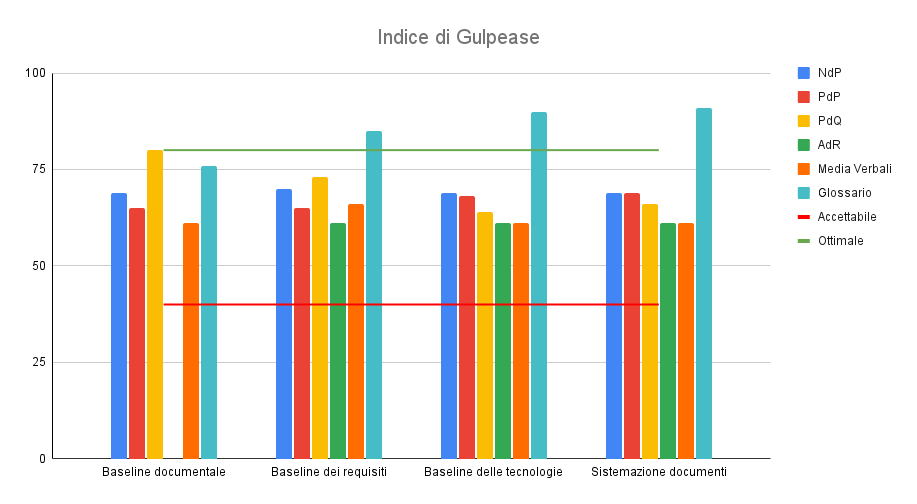
\includegraphics[width=0.8\textwidth, height=0.8\textheight,keepaspectratio]{images/RTB-Indice-di-Gulpease.png}
    \caption{Grafico dell'indice di Gulpease dei documenti nelle varie fasi dell'RTB.}
\end{figure}    

\subsubsection{M15VC - Variazione di Costo}
\begin{figure}[H]
    \centering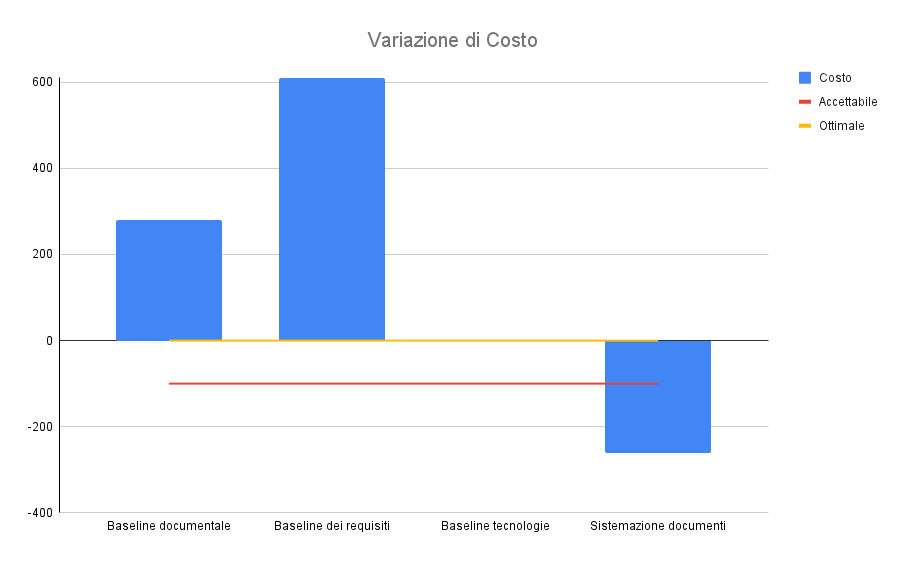
\includegraphics[width=0.8\textwidth, height=0.8\textheight,keepaspectratio]{images/RTB-Variazione-di-Costo.png}
    \caption{Grafico che indica come sono variati i costi rispetto a quelli preventivati nelle varie fasi dell'RTB.}
\end{figure}    

\subsubsection{M16VP - Variazione di Piano}
\begin{figure}[H]
    \centering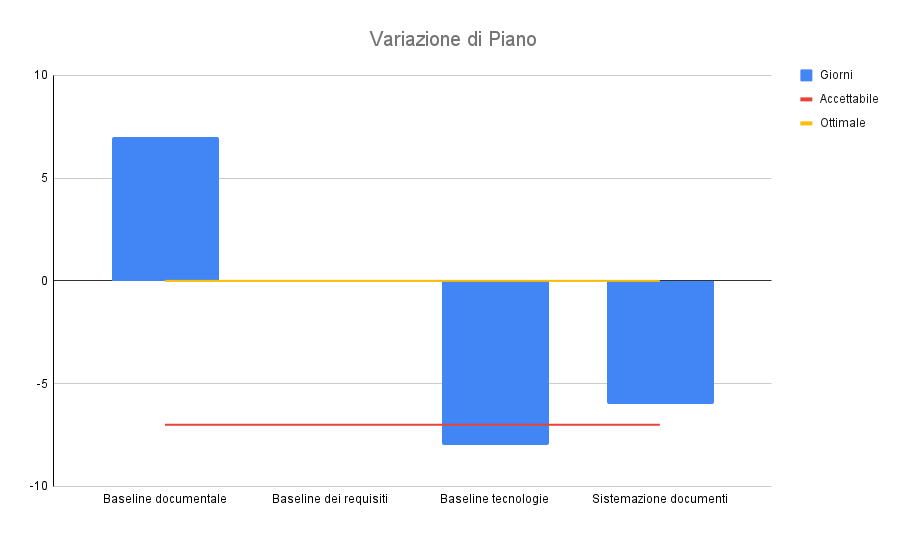
\includegraphics[width=0.8\textwidth, height=0.8\textheight,keepaspectratio]{images/RTB-Variazione-di-Piano.png}
    \caption{Grafico che indica come è variata la pianficazione rispetto al preventivo nelle varie fasi dell'RTB.}
\end{figure}  


\subsection{Macrofase PB}
\subsubsection{M14IG - Indice di Gulpease}
\begin{figure}[H]
    \centering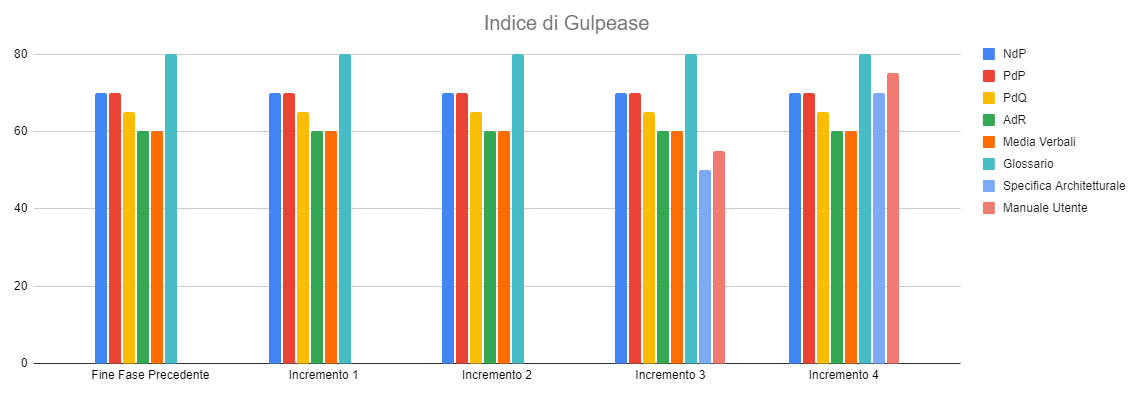
\includegraphics[width=\textwidth, height=\textheight,keepaspectratio]{images/PB-Indice-di-Gulpease.png}
    \caption{Grafico dell'indice di Gulpease dei documenti nelle varie fasi della PB.}
\end{figure}    

\subsubsection{M15VC - Variazione di Costo}
\begin{figure}[H]
    \centering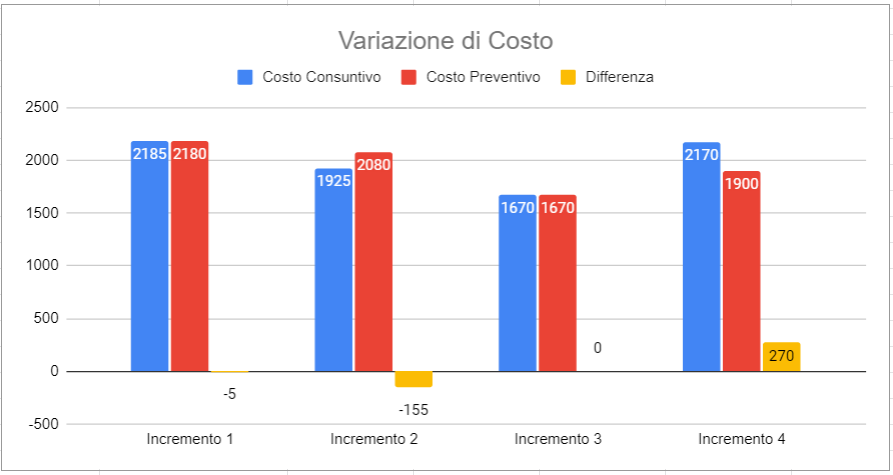
\includegraphics[width=0.8\textwidth, height=0.8\textheight,keepaspectratio]{images/PB-Variazione-di-Costo-2.png}
    \caption{Grafico che indica come sono variati i costi rispetto a quelli preventivati nelle varie fasi della PB.}
\end{figure}    

\subsubsection{M16VP - Variazione di Piano}
\begin{figure}[H]
    \centering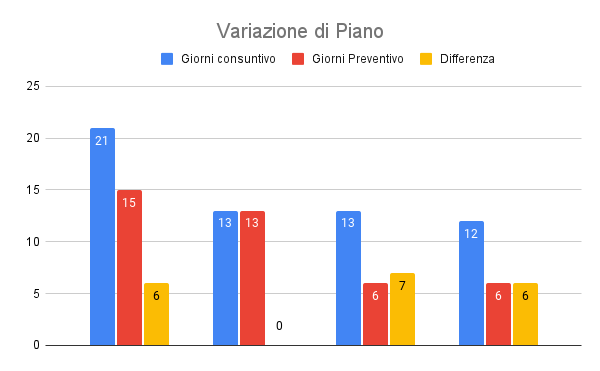
\includegraphics[width=0.8\textwidth, height=0.8\textheight,keepaspectratio]{images/PB-Variazione-di-Piano-3.png}
    \caption{Grafico che indica come è variata la pianificazione rispetto al preventivo nelle varie fasi della PB.}
\end{figure}  

\subsubsection{M8CC - Code Coverage}
\begin{figure}[H]
    \centering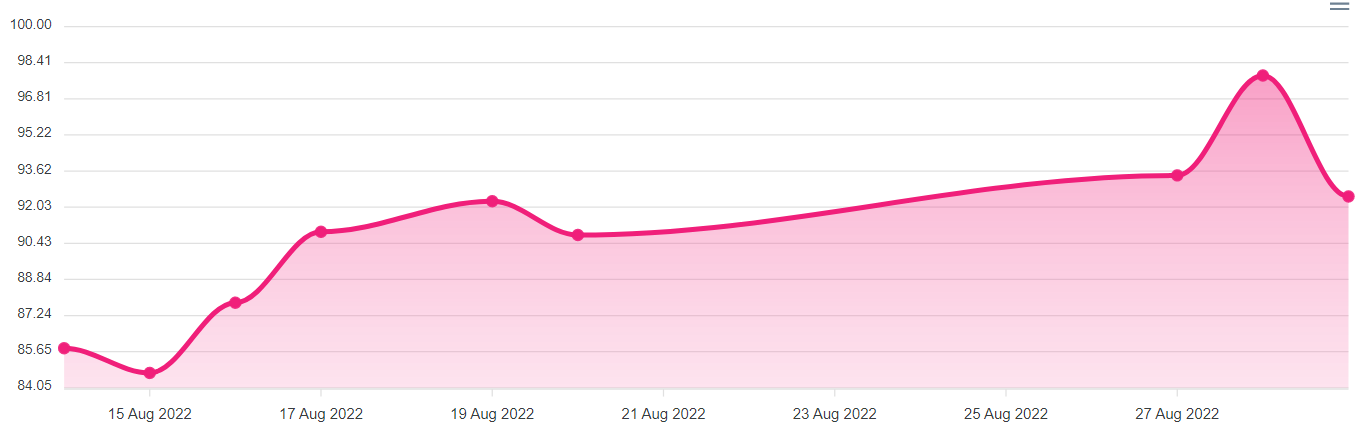
\includegraphics[width=0.8\textwidth, height=0.8\textheight,keepaspectratio]{images/PB-Code-Coverage.png}
    \caption{Grafico che indica come è variata la percentuale di codice coperto da Test nel corso del progetto.}
\end{figure}  

\subsubsection{M1PRR - Percentuale di Requisiti Obbligatori Soddisfatti}
\begin{figure}[H]
    \centering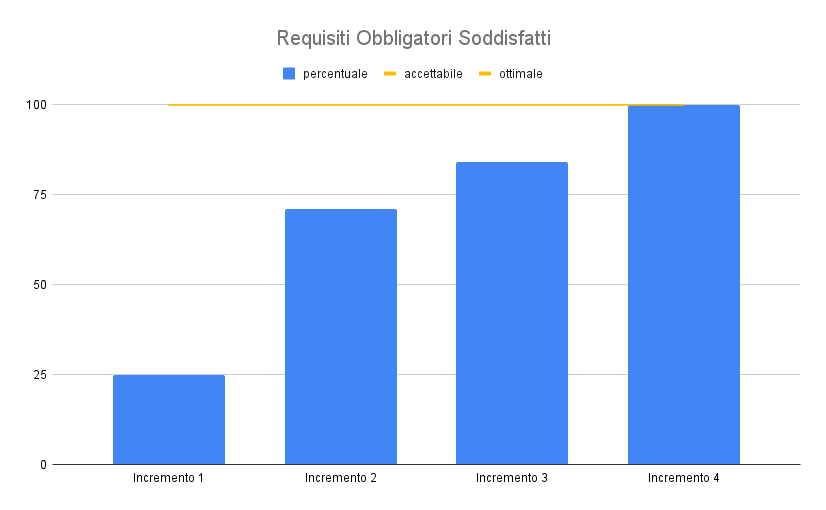
\includegraphics[width=0.8\textwidth, height=0.8\textheight,keepaspectratio]{images/PB-Requisiti-Obbligatori-Soddisfatti.png}
    \caption{Grafico che indica come è variata la percentuale di requisiti obbligatori soddisfatti.}
\end{figure}  

\subsubsection{M2PDR - Percentuale di Requisiti Desiderabili Soddisfatti}
\begin{figure}[H]
    \centering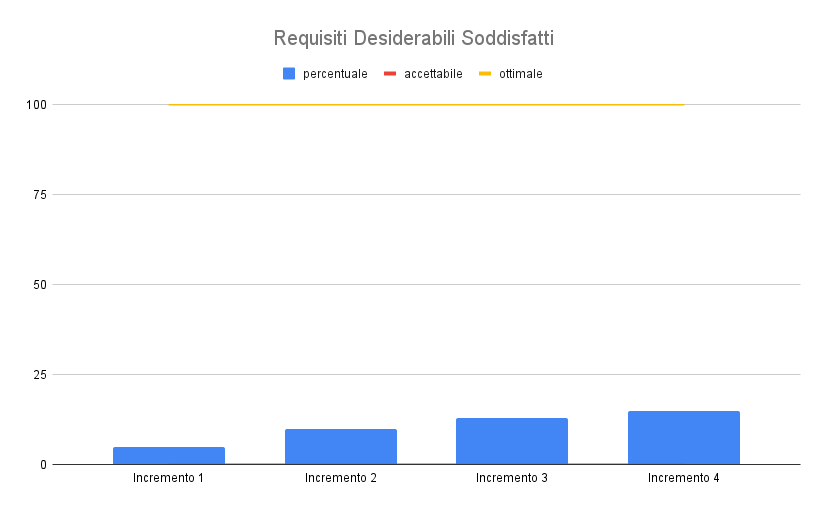
\includegraphics[width=0.8\textwidth, height=0.8\textheight,keepaspectratio]{images/PB-Requisiti-Desiderabili-Soddisfatti.png}
    \caption{Grafico che indica come è variata la percentuale di requisiti desiderabili soddisfatti.}
\end{figure}  
\end{document}